\documentclass{article}
\usepackage{amsmath,amssymb}
\usepackage{fullpage}
\usepackage{enumerate}
\usepackage{tikz}

\newcommand{\dsum}{\displaystyle\sum}
\newcommand{\dint}{\displaystyle\int}
\newcommand{\abs}[1]{\displaystyle\left\lvert#1\right\rvert}
\newcommand{\dbcup}{\displaystyle\bigcup}
\newcommand{\dbcap}{\displaystyle\bigcap}
\newcommand{\dcup}{\displaystyle\cup}
\newcommand{\dcap}{\displaystyle\cap}
\newcommand{\Pb}{\mathbb{P}}
\newcommand{\Eb}{\mathbb{E}}
\newcommand{\bkt}[1]{\left(#1\right)}
\title{MA2040: Probability, Statistics and Stochastic Processes\\
Problem Set-III}
\author{Sivaram Ambikasaran}
\begin{document}
	\maketitle
	\begin{enumerate}
		\item
		If $X_1,X_2,\ldots,X_n$ are independent random variables having the same probability density function $f_X(x)$, what is the probability density function for the random variable $Y=\text{min}\{X_1,X_2,\ldots,X_n\}$?
		\item
		A random variable $X$ has a probability density function as shown below.
		\begin{center}
		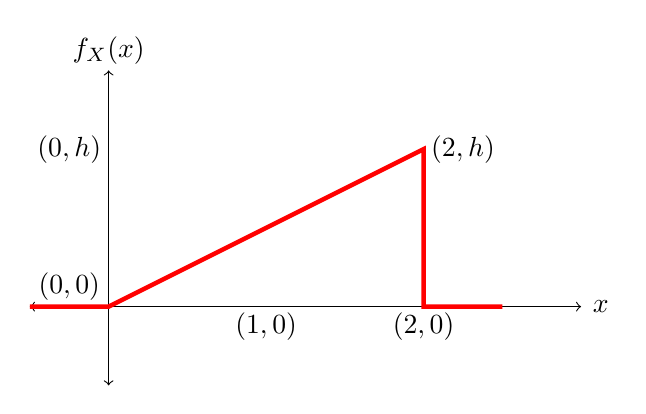
\begin{tikzpicture}[scale=2]
			\draw [<->] (-0.5,0) -- (3,0);
			\draw [<->] (0,-0.5) -- (0,1.5);
			\node at (3.125,0) {$x$};
			\node at (0,1.625) {$f_X(x)$};
			\draw [ultra thick,red] (-0.5,0) -- (0,0) -- (2,1) -- (2,0) -- (2.5,0);
			\node at (-0.25,0.125) {$(0,0)$};
			\node at (1,-0.125) {$(1,0)$};
			\node at (2,-0.125) {$(2,0)$};
			\node at (-0.25,1) {$(0,h)$};
			\node at (2.25,1) {$(2,h)$};
		\end{tikzpicture}
		\end{center}
		\begin{enumerate}
			\item
			Determine $h$
			\item
			Determine the cummulative distribution function
			\item
			Compute the mean
			\item
			Compute the variance
			\item
			Determine the probability that $X \in \bkt{1,2}$.
		\end{enumerate}
		\item
		The median $m$ of a probability density function is defined as the value of $m$ such that
		$$\dint_{-\infty}^m f(x) dx = \dint_m^{\infty} f(x) dx =1/2$$
		Essentially, the median splits the distribution into two equal halves. Prove that the median is the best predictor if one wants to minimize the expected value of the absolute error, i.e., $\mathbb{E}\bkt{\abs{X-c}}$ is minimized when $c$ is the median of the underlying distribution.
		\item
		Let $X$ be a random variable, whose pdf is given by
		$$f_X(x) = \begin{cases}
		0 & \text{ if }x \leq 0\\
		xe^{-x^2/2} & \text{ if }x>0
		\end{cases}$$
		Find the pdf for the random variable $Y=X^2$.
		\item
		Let $X$ be a uniform random variable on the interval $[0,1]$. Consider the random variable $Y=g\bkt{X}$, where
		$$g(x) = \begin{cases}
		1 & \text{ if }x \leq 1/3\\
		2 & \text{ else}
		\end{cases}$$
		Find the probability mass function of $Y$ and compute its expected value.
		\item
		Show the expected value of a random variable $X$ can also be obtained as
		$$\Eb\bkt{X} = \dint_0^{\infty} \Pb \bkt{X > x}dx - \dint_0^{\infty} \Pb\bkt{X < -x}dx$$
		\item
		A defective coin minting machine produces coins whose probability of heads is a random variable $Y$ with PDF
		$$f_Y\bkt{y} = \begin{cases}
		y \exp\bkt{y} & \text{ if }y \in [0,1]\\
		0 & \text{ otherwise}
		\end{cases}$$
		A coin produced by this machine is selected and tossed repeatedly, with successive tosses assumed independent.
		\begin{enumerate}
			\item
			Find the probability that a coin toss results in head.
			\item
			Given that a coin toss resulted in heads, find the conditional PDF of $Y$.
			\item
			Given that the first coin toss resulted in heads, find the conditional probability of heads on the next toss.
		\end{enumerate}
		\item
		Let the randomvariables $X$ and $Y$ have a joint PDF, which is uniform over the triangles with vertices $(0,0)$, $(0,1)$ and $(1,0)$.
		\begin{enumerate}
			\item
			Find the joint PDF of $X$ and $Y$.
			\item
			Find the marginal PDFs.
			\item
			Find the conditional PDFs.
		\end{enumerate}
		\item
		Chennai's temperature is modeled as a normal random variable with a mean temperature of $34^{\circ}$C and a standard deviation of $5^{\circ}$C. What is the probability that the temperature at a randomly chosen time will exceed $45^{\circ}$C?
		\item
		A surface is ruled with parallel lines, which are at a distance $d$ from each other. Suppose that we throw a needle of length $l$ on the surface at random. What is the probability that the needle with intersect one of the lines? (NOTE: You will need to treat the case $d<l$ and $d>l$ separately.)
		\item
		Consider two continuous random variables $Y$ and $Z$ and a random variable $X$ that is equal to $Y$ with a probability $p$ and equals $Z$ with a probability $1-p$. Obtain the pdf of $X$ interms of the pdf's of $Y$ and $Z$.
	\end{enumerate}
\end{document}